% \documentclass[]{amsbook}
\documentclass[]{article}

% \input MyMacros.tex

\usepackage{graphicx}% Include figure files
\usepackage{dcolumn}% Align table columns on decimal point
\usepackage{bm}% bold math
% \usepackage{pictex}%
\usepackage{verbatim} % this is needed for \begin{comment} ... \end{comment}
\usepackage{lscape} % this is needed for occasional landscape figures
\usepackage{amsmath}
% \usepackage{appendix}
% \usepackage{subfigure}
\usepackage{epsfig}
\usepackage{amsfonts}
\usepackage[margin=1.1in, top=1.1in, bottom=1.1in]{geometry}

% \textwidth 550pt
% \textheight 500pt
% \hoffset -3.5cm
\def\betabold{{\pmb{$\beta$}}}

\setcounter{tocdepth}{3}
%
\begin{document}

\date{July 21, 2014}

% \voffset=1.5
\title{
\centerline{}
\centerline{}
\centerline{}
UAL/ETEAPOT Benchmark Comparisons V: \\ 
Spin Evolution in an All-Electric Lattice
Coasting Beam}
\author{J. D. Talman and R. M. Talman
}

\maketitle

%
\begin{abstract}
The main purpose for this report is to document the treatment of
spin evolution by UAL/ETEAPOT (\#ual1127). By this time ETEAPOT supports
bunched beam spin evolution but, for this report, there is
no RF cavity and no synchrotron oscillations. With no RF cavity in 
the ring, only coasting, not bunched, beams can be modeled. 
Since long spin correlation time (SCT) can only be achieved with 
bunched beams, the tracking described here can determine parameters 
affecting 
SCT but cannot obtain usefully long SCT values directly. Direct 
determination of bunched beam SCT values using ETEAPOT will be 
the subject for a ``Benchmark Comparisons-VI'' report.

For the present report, a new lattice called {\tt E\_Protonium.sxf}
(with $m=0$ and $m=1$ variants) is introduced and tracked.
``$m$=1 protonium'' is a hypothetical atom consisting of a 
single proton bound to an infinite mass charged particle at the 
origin; the charge is just right so that a proton having the 
magic frozen spin momentum can travel in a circle of radius $r_0=40\,$m, 
which is the radius of the nominal proton EDM lattice. 
``$m$=0 protonium'' is the same except the central charge is a fixed
line charge of the correct strength for magic momentum protons
to be bound in a circle of the same $r_0=40\,$m radius.

There is no pretense that ``protonium'' is a physically useful
or even realizable atom, nor is there pretense that the
lattice can serve as a practical EDM apparatus.
Though structured with a large number of (identical) bending 
elements, all drift lengths are set nearly to zero. What is left
is a physical system all of whose parameters, in particular
SCT, can be calculated analytically, with orbits close to the
design orbit treated either analytically or perturbatively. 
This provides the
simplest possible configuration for testing the reliability
of the code and for comparison with other codes.

The ``physics'' emphasis in this report is on comparing $m=1$ and $m=0$
spin evolution. One significant observation is a four orders
of magnitude greater spin decoherence with $m=1$ than with $m=0$,
admittedly in a special case. Preliminary tracking showed that
nearly circular orbits were subject to spurious damping, but this
was fixed by more careful numerical treatment. With this
more careful treatment there is still a hint of horizontal
(anti-)damping in the $m=0$ case. Fortunately the doubling 
time is sufficiently long (about 100,000 turns) that this growth,
though probably unphysical, is small enough to be ignored 
when studying spin decoherence.
\end{abstract}
%

\clearpage

\tableofcontents

\clearpage

\section{Tracking Results and Interpretation}
\subsection{Introduction}
The initial part of this report contains ETEAPOT spin tracking results
and tentative explanation of them. Lengthier and more technical 
documentation of the code is contained in appendicies. Only two
lattices are analysed and both are highly idealized, primarily
by having bends separated only by negligibly short straight sections
and by having extremely weak quadrupoles, just strong enough
for betatron motion in both planes to be stable. One lattice
is ``cylindrical'' or $m=0$, the other is ``spherical'' or $m=1$.
To encourage the reader to think of an electric accelerator storage ring
as not essentially different from an atom, these lattices are referred
to as two variants of a hypothetical atom called ``protonium'',
with a single proton bound to a fixed line charge or point charge. 
 
\subsection{Parameters and Twiss Functions of the ``Protonium'' Lattices}
%
\begin{table}[h]
\caption{\label{tbl:ProtoniumParams}For $m$=1 the force field is central, which makes
the design orbit degenerate---every circular orbit with the design energy is 
congruent to an equatorial orbit.
This causes $Q_y$ in the $m$=1 case to be ambiguous; with the design orbit \emph{defined}
to lie in the horizontal plane, a particle with initial vertical offset is interpreted
as having $Q_y$=1, in spite of the fact that its orbit lies in a single (slanted) plane, 
and is congruent to the design orbit. For the $m$=0, cylindrical case, tiny vertically 
focusing quads of strength $q$, are inserted to restore marginal stability. The
source of the ``indeterminate'' entry in one case is a nuisance associated with inverse trig
functions, with vertical tune extremely small and vertical beta function extremely
large. Otherwise there is excellent agreement between two independent codes concerning
the standard lattice functions.} 
\medskip
\centering
\begin{tabular}{|c|c|c|c|c|c|c|c|}           \hline
file name           & variable name     & unit &   $m$=0, cylindrical  &  $m$=1, spherical   \\ \hline
cells/arc           & {\tt NCellPerArc} &      &      20               &       20            \\
bend radius         &  {\tt r0}         &  m   &     40.0              &      40.0           \\
half drift length   &  {\tt Ldh}        &  m   &   $10^{-6}$            &   $10^{-6}$         \\
half bend per cell  & {\tt Thetah}      &  r   &   0.078539816         &  0.078539816        \\
half bend length    & {\tt Leh}         &  m   &    3.141592           &  3.141592           \\
circumference       & {\tt circum}      &  m   &    251.327            &   251.327           \\ \hline
inv. focal length   &  {\tt q}          & 1/m  &    1.0e-6             &  1.0e-6(effective)  \\
field index         &  {\tt m}          &      &      0.0              &    1.0              \\ \hline
%
horz. beta(MAPLE)   & {\tt betax}       &  m   &     31.24             &   49.92             \\
horz. beta(ETEAPOT) &                   &  m   &     31.19             &   49.92             \\ \hline
%
vert. beta(MAPLE)   & {\tt betay}       &  m   &    1772               &   40.00             \\ 
vert. beta(ETEAPOT) &                   &  m   &    1765               & indeterminate       \\ \hline
%
horz. tune(MAPLE)   &  {\tt Qx}         &      &    1.2813             &   0.8012            \\
horz. tune(ETEAPOT) &                   &      &    1.2815             &   0.8012            \\ \hline
%
vert. tune(MAPLE)   &  {\tt Qy}         &      &    0.0225            &   1.0000            \\ 
vert. tune(ETEAPOT) &                   &      &    0.0226            &   1.0000            \\
\hline
\end{tabular}
\end{table}
%

\subsection{Simplifications}
This report documents spin evolution of polarized protons as
predicted by ETEAPOT. It is preliminary and over-simplified
in two ways compared to the spin tracking that will eventually
be required for the proton EDM measurement. 

One oversimplification is the restriction to coasting beams---with 
no RF cavitities there is no longitudinal acceleration and any
spread of injection energy will cause the coasting beam to spread 
longitudinally. Spin coherence times (SCT) obtained this way are
expected to be far too short to permit realistic EDM measurements;
it is only with synchrotron oscillation averaging that 
acceptably long SCT values can be expected. The purpose for the present
preliminary tracking is to quantify the SCT contributions due to various 
initial phase space offsets from the design orbit.

The other simplification is that the lattice will be ``all bends''
with no straight sections. In numerical treatments like ETEAPOT, the
presence of absence of straight sections is of little consequence.
But for analytic precession calculations the presence of straight 
sections provides undesirable complication. To better motivate analytic
calculations, and as a mnemonic, we refer to the drift-free lattice 
as ``protonium''. Analytic treatment of the protonium atom can then 
be compared with numerical treatment of the same system 
treated as an accelerator lattice.

\subsection{Cautionary Comments}
The drift lengths in the {\tt E\_Protonium.sxf} lattice are negligibly
short compared to electrode separation ``$gap$''. This is opposite to
the usual situation, in which drift lengths are long compared to
fringe field lengths, which is what ETEAPOT assumes by default. So, for 
investigating protonium, the fringe field correction has to be set to 
zero in the code.  

In this report, the contributions to spin precession for various
initial phase space displacements differing from zero are obtained. 
All six coordinates are treated on equal terms. This is misleading as regards
interpretation of the relative importance of transverse and
longitudinal initial offsets. Nevertheless, ignoring this distinction, 
reading from plots shown later, entries are made in 
Table~\ref{tbl:ExcessPrecessions}, and interpreted as spin coherence
times due to the various offsets.
%
\begin{table}[h]
\caption{\label{tbl:ExcessPrecessions}Excess precession caused by various
initial phase space conditions for the particles being tracked. The entries
are obtained from Figures~\ref{fig:SpinEvolve11.12} through 
\ref{fig:SpinEvolve0.17}. One notes that all SCT values in the table are 
very short compared to
the nominal target value of SCT=1000\,s desired for the proton EDM experiment.
But the results shown here are for coasting beams; for bunched beams there 
will be energy averaging accompanying synchrotron oscillations 
that can be expected to increase the SCT values by, perhaps,
two orders of magnitude. Excess precession for examples in the 
first six rows are expected to be quadratic in initial coordinate
offset. Only for the final two rows are
the excess precessions expected to be linear in the initial
coordinate offset. 
Especially noteworthy is the dramatic difference between SCT values
due to energy offset in the cylindrical and spherical cases; i.e. the two 
bottom rows. This is discussed below.
} 
\medskip
\centering
\begin{tabular}{|c|c|c|c|c|}           \hline
initial offsets       & $\Delta s_x$/turn[Z] & SCT[Z] & $\Delta s_x$/turn[P1.0] & SCT[P1.0] \\
                      &                      & ``cylindrical'' &         & ``spherical''    \\
                      &                      &      s      &             &   s  \\ \hline
%
 0.0005 0 0 0 0 0     &    -1.1e-7           &   9         &    -1.6e-7  &   7      \\
-0.0005 0 0 0 0 0     &    -1.1e-7           &   9         &    -1.6e-7  &   7      \\
 0  0.0002 0 0 0 0 0  &    -1.6e-7           &   6         &    -6.2e-7  &  1.6      \\
 0 -0.0002 0 0 0 0 0  &    -1.6e-7           &   6         &    -6.2e-7  &  1.6     \\
 0 0 0.01 0 0 0       &     1.8e-7           &  5.5        &     2.5e-7  &  0.4     \\
 0 0 0 0.01 0         &     N/A              &  N/A        &     3.7e-6  &  0.24    \\ \hline
 0.01 0 0 0 0 5.85e-5 &    -4.8e-7           &  2.1        &     1.4e-3  &  0.0007  \\
 0 0 0 0 0 5.85e-5    &    -4.6e-7           &  2.2        &     1.4e-3  &  0.0007  \\
\hline
\end{tabular}
\end{table}
%

By up-down symmetry, the excess precession $\Delta s_x/{\rm turn}$ has
no contribution proportional to either $y_0$ or $y'_0$. The leading 
vertically-induced decoherence
is proportional to $\epsilon_{y,CS}$, the (generalized) vertical Courant-Snyder
invariant, which is quadratic in $y_0$ and $y'_0$. Horizontal betatron
oscillations are similarly proportional to the horizontal invariant 
$\epsilon_{x,CS}$ (though there is also the possibility of contributions
depending on $x_0$ or $x'_0$ multiplied by energy offset
$\Delta\mathcal{E}$). But decoherence due to initial energy offset 
$\Delta\mathcal{E}$ is different. There will
be excess precession linear in $\Delta\mathcal{E}$ . In spite
of these differences, for semi-quantitative comparison 
in Table~\ref{tbl:ExcessPrecessions}, because all
8 particles have ``typical'' amplitudes, their contributions to SCT are
simply quoted as the excess precession per turn divided by the
time per turn.  

A possible source of confusion is that particle energies in
ETEAPOT are established \emph{outside} bend elements; i.e. positions
where the electric potential vanishes. This continues
to be true for protonium, even though the particles are almost
never outside bend elements. Bend elements are treated as having
``hard'' edges, meaning the electric potential changes discontinuously 
from zero outside, to non-zero inside. The drift lengths, though short, 
e.g. 1 micrometer, are not exactly zero. Particle energies are
assigned, and subsequently evaluated, within the drift sections.
Of course the total particle energy, mechanical (rest energy plus
kinetic energy) plus potential is conserved (except in RF cavities
of which there are none at present), so the discontinuous 
change of potential energy causes a cancelling change in kinetic 
energy. For straight sections of negligible length
the net fringe field effect as a particle proceeds from just 
before exiting a bend element to just after entering the next one
can be neglected.

\subsection{Protonium}
As introduced in the abstract, ``protonium'' is an imaginary atom
formed from a single proton bound to a fixed (i.e. infinite
mass) negative point charge situated at the origin. With the
proton anomalous magnetic moment being $G=1.79284736$, the magic
momentum is $p_0c=0.7007405364\,$GeV, the velocity is 
$0.598379077 c$ and radial electric field
$E_m$ required to give a circular orbit of radius $r_0=40\,$m is
%
\begin{equation}
E_m 
 = 
\frac{(m\gamma_0v/e)\beta_0c}{r_0} 
 =
\frac{(p_0c/e)\beta_0c}{r_0}
 =
0.0104827119\,{\rm GV/m}.
\label{eq:Protonium.1}
\end{equation}
% 
The charge $Q_{m=1}$ giving this electric field at distance $r_0$ is 
%
\begin{equation}
Q_{m=1}
 =
4\pi\epsilon_0r_0^2E_m
 =
1.866174\,{\rm C}.
\label{eq:Protonium.2}
\end{equation}
% 
The corresponding line charge density $\lambda_{m=0}$ for $m=0$ is  
%
\begin{equation}
\lambda_{m=1}
 =
2\pi\epsilon_0r_0E_m
 =
0.023327180\,{\rm C/m}.
\label{eq:Protonium.3}
\end{equation}
%
To produce orbits close to the design circular orbit, ETEAPOT
treats the protonium as an accelerator lattice consisting of
a large number (such as 80 elements, each bending through
$2\pi/80$) separated by straight sections of negligible length.

\section{Coasting Beam Spin Precession in Idealized Rings}
\subsection{Spin Evolution}
The following series of figures compare spin evolution 
(actually just the transverse spin component $s_x\equiv s[0]$) for
various particles all having initial spin purely longitudinal
(where ``longitudinal means ``along the tangent to the design orbit''
\emph{not} ``along the particle's orbit''.

Initial phase space coordinates are indicated at the top
of each graph in the form 
{\tt Z (or P1.0): x\_0, x'\_0, y\_0, y'\_0, ct\_0, 
$\Delta\mathcal{E}$\_0/(p\_0c)},
where {\tt Z} stands for $m=0$, ``cylindrical'' electrodes,
and {\tt P1.0} stands for $m=1.0$, ``spherical''
electrodes. Very weak vertically focusing quads, of strength $q$ 
given in the parameter table, provide just enough vertical focusing 
so that orbits are stable vertically.
With weak vertical focusing the $m=0$ case is barely stable 
vertically, causing particles with too great vertical momenentum
to be lost.

\bigskip

\noindent
{\bf Hint concerning running the code:} Initial conditions for the 21 (or any
other number of particles being tracked) are given in the {\tt userBunch} file,
an example of which is given in an appendix. 
\bigskip
%
\begin{figure}[h]
\centering
\includegraphics[scale=0.6]{eps/SpinEvolve11.Z.eps}
\includegraphics[scale=0.6]{eps/SpinEvolve11.P1.0.eps}
\includegraphics[scale=0.6]{eps/SpinEvolve12.Z.eps}
\includegraphics[scale=0.6]{eps/SpinEvolve12.P1.0.eps}
\caption{\label{fig:SpinEvolve11.12}The figures on the left have 
$m=0$, those on the right have $m=1$. The upper/lower figures
have initial horizontal displacements $x_0=\pm5\,$mm, and all other
initial displacements zero. The dashed lines are fits to 
the right graph copied to the left. 
}
\end{figure}
%

%
\begin{figure}[h]
\centering
\includegraphics[scale=0.6]{eps/SpinEvolve13.Z.eps}
\includegraphics[scale=0.6]{eps/SpinEvolve13.P1.0.eps}
\includegraphics[scale=0.6]{eps/SpinEvolve14.Z.eps}
\includegraphics[scale=0.6]{eps/SpinEvolve14.P1.0.eps}
\caption{\label{fig:SpinEvolve13.14}The figures on the left have 
$m=0$, those on the right have $m=1$. The upper/lower figures
have initial horizontal slopes $x'_0=\pm0.0002$, and all other
initial displacements zero. The dashed lines are fits to
the right graph copied to the left. 
}
\end{figure}
%
The graphs of Figure~\ref{fig:SpinEvolve11.12} indicate  
that the spin precession accompanying initial horizontal
displacement depends only weakly on the value of $m$.
The graphs of Figure~\ref{fig:SpinEvolve13.14} 
show the precession accompanying initial horizontal
slope somewhat greater with $m$=1 than with $m$=0.

The graphs may
seem, superficially, to contradict the assumption that the
spins are purely longitudinal initially. But betatron oscillations
rapidly produce small transverse spin components of the same order
as the betatron slope components.

\clearpage

%
\begin{figure}[h]
\centering
\includegraphics[scale=0.6]{eps/SpinEvolve15.Z.eps}
\includegraphics[scale=0.6]{eps/SpinEvolve15.P1.0.eps}
\includegraphics[scale=0.6]{eps/SpinEvolve16.Z.eps}
\includegraphics[scale=0.6]{eps/SpinEvolve16.P1.0.eps}
\caption{\label{fig:SpinEvolve15.16}The figures on the left have 
$m=0$, those on the right have $m=1$. The upper figures
have initial vertical displacement $y_0=0.01$, and all other
initial displacements zero.  The lower figures
have initial vertical slope $y'_0=0.001$, and all other
initial displacements zero. The dashed lines are fits to
the right graph copied to the left. (Because there is
only extremely weak
vertical focusing in the $m=1$ case, the vertical displacement
rapidly increases beyond the ETEAPOT default aperture of 1\,m
in \emph{the lower left graph, which therefore has to be ignored}.)
}
\end{figure}
%
Figure~\ref{fig:SpinEvolve15.16} shows dependence on initial
vertical displacements and slopes. For consistency there is
the same left/right graph organization of graphs.
But the lower left graph has to be ignored because the
$m=0$ lattice is insufficiently stable vertically. 
By default treatment in ETEAPOT, particle transverse positions 
are not allowed to exceed 1 meter; this occurs after just a 
few turns with the initial vertical slope being 0.001.

Figure~\ref{fig:SpinEvolve0.17} shows dependence on initial
energy offset, for two initial radial offsets. Again, the
graphs on the left are for cylindrical, on the right for
spherical. The excess precessions in the $m$=1 spherical case are
so great that the spin makes about three complete revolutions
relative to the particle momentum during the 10,000 turns
shown; this is shown by the sinusoidal variation of $s_x$
between +1 and -1.
Yet the excess precession for a particle with the same initial
conditions is barely visible in the $m$=0 cylindrical case.

This four order of magnitude difference in excess precession is, 
by far, the most striking observation in the report---enough so 
as to be discussed further below.
%
\begin{figure}[h]
\centering
\includegraphics[scale=0.6]{eps/SpinEvolve0.Z.eps}
\includegraphics[scale=0.6]{eps/SpinEvolve0.P1.0.eps}
\includegraphics[scale=0.6]{eps/SpinEvolve17.Z.eps}
\includegraphics[scale=0.6]{eps/SpinEvolve17.P1.0.eps}
\caption{\label{fig:SpinEvolve0.17}The figures on the left have 
$m=0$, those on the right have $m=1$. The upper figures
have initial horizontal displacement $1\,$cm and fractional
off-energy displacement 5.85e-5; these displacements are 
matched to cause the subsequent orbit to be exactly a circle 
of radius 1\,cm greater than the design orbit in the $m=1$
protonium case (but not in the $m=0$ cylindrical case). 
The lower figure
has the same energy offset but vanishing initial horizontal
displacement. The dashed lines are fits to
the right graph copied to the left. Note that the precession
rate is so much greater for the $m$=1 (spherical) case,
than for the $m$=0 (cylindrical) that the dashed lines
are just barely visible in plots on the left, even with
the vertical range so great that the precession in the
$m=0$ case is itself barely visible. All by themselves these
plots make the case for the superiority of $m$=0 over $m$=1 for
long spin coherence time.
}
\end{figure}
%

\clearpage

The particular choice of initial conditions;
$(x_0, x_0', y_0, y_0', ct_0, \Delta\mathcal{E}/(p_0c))$ = 
$(0.01, 0, 0, 0, 0, 5.85e$-5)
was not arbitrary. Rather, the value $\Delta\mathcal{E}/(p_0c)=5.85$e-5
is exactly the energy offset for which a particle will travel exactly 
in a circle of radius $40.01\,$m in the $m$=1 spherical lattice. 
This corresponds to a calculable offset $\Delta\gamma=\gamma-\gamma_0$ 
relative to the magic (or design) value $\gamma_0$. 
This behavior is confirmed by ETEAPOT, in the upper right graph of
Figure~\ref{fig:xEvolve0}. Then, because the velocity 
is permanently offset by an appreciable amount, it is not surprising 
that the excess spin precession is large 
(i.e. three complete revolutions in 10,000 turns).
The initial energy offset was not exactly correct but, noting the
exceedingly expanded scale, it was close.

The upper left figure shows the off-momentum evolution 
of the same particle in the $m=0$ cylindrical lattice.
The orbit oscillates about the circle for which $x=0.004\,$m.
All that is left is to apply conservation of energy, along with the
known dispersion in the $m=0$ lattice, to check that this is
the appropriate central orbit, and then to figure out what its
excess spin precession should then be. Actually it is simpler than this,
because we know that \emph{all}  circular orbits in the cylindrical 
case have the magic velocity. If, on the average, the orbit is 
circular, then its average velocity is necessarily magic, and its 
excess precession close to zero.
 
With the initial energy offset not quite correct, one expects 
a particle to execute tiny perpetual oscillations
about a central value such as $x=0.01\,$m (on the right)
or $x=0.004\,$m (on the left). As mentioned in the abstract, 
in a preliminary version of this report,
nearly circular orbits such as these exhibited spurious damping onto 
exactly circular orbits. More careful numerical treatment 
has reduced this damping by more than two orders of magnitude. This 
improvement was not accomplished by artificial ``symplectification'', 
which is a device some programs employ to ameliorate spurious damping
or anti-damping. Rather it came from more careful
treatment of the approximate cancellation occurring in subractions 
such as $r-r_0$, having a value of order one centimeter with $r_0=40\,$m.

It is expected that (in more realistic lattices, with bunched beams, 
and sextupole compensation) run durations of $10^4$ or $10^5$ turns 
should be long enough to provide adequate calculation of spin coherence 
times (SCT), even though the run durations in an actual EDM experiment 
need to be about $10^9$ turns. As well as requiring parallel processing,
computer simulation of such long runs will require either more accurate
numerical processing or artificial symplectification, or both.

Comparing figures on the left and on the right 
of Figure~\ref{fig:xEvolve0}, one sees that 
residual damping in the $m=0$ case exceeds that in the $m=1$ case
by an order of magnitude. This could be due to amplitude dependence,
since the radial oscillation amplitude is much greater on the left. Even
with no synchrotron oscillations, in the all-electric lattice, radial
oscillations are accompanied by speed oscillations which mix radial
and longitudinal oscillations. The dependence on $m$ might also
be due to resonant enhancement of numerical errors which depends on 
the horizontal tune.

Tempering enthusiasm for the $m=0$ lattice is the fact that 
the injection acceptance into the cylindrical lattice is extremely small, 
which obviously limits the number of protons that can be stored.
Also, according to Valeri Lebedev's calculations, beam growth due
to intrabeam scattering is especially rapid for weak focusing,
low energy, proton lattices.

%
\begin{figure}[h]
\centering
\includegraphics[scale=0.5]{eps/xEvolve0.Z.eps}
\includegraphics[scale=0.5]{eps/xEvolve0.P1.0.eps}
\includegraphics[scale=0.5]{eps/xEvolve0.Z-200turn.eps}
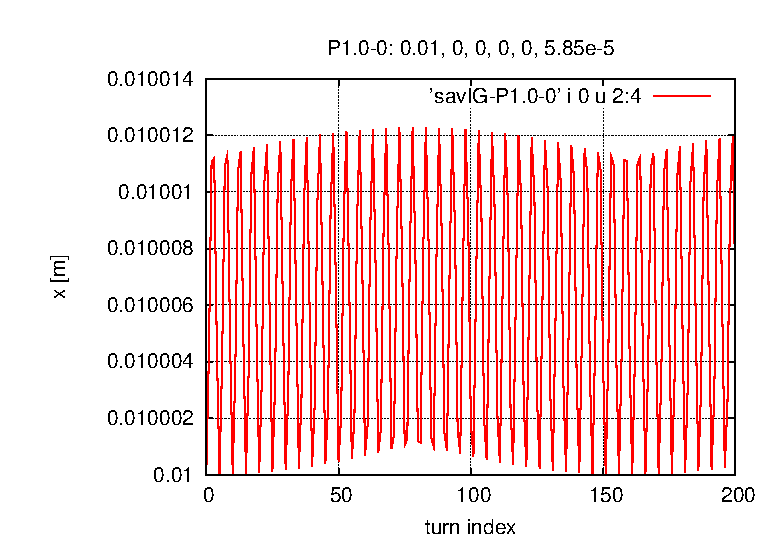
\includegraphics[scale=0.5]{eps/xEvolve0.P1.0-200turn.eps}
\caption{\label{fig:xEvolve0}In these plots radial displacements $x$
are plotted against turn number. The lower plots zoom in on the
first 200 turns. As in previous figures the $m$=0, cylindrical
plots are on the left, the $m$=1, spherical
plots are on the right. In a preliminary version of this report
the upper curves damped to perfect circles over 100's of turns,
as the lower graphs showed. More careful numerical treatment all 
but eliminated this spurious damping by more than two orders
of magnitude. Some (anti-)damping, presumeably still spurious,
remains, though only in the $m=0$ case.
}
\end{figure}
%

\clearpage

\appendix

\section{Spin Tracking in ETEAPOT}
\subsection{Approximations}
%
\begin{itemize}
\item
To leading approximation all spin precession occurs in central force,
inverse square law, ``Kepler force'' regions. With this assumption
the orbit through a bend element of any individual particle lies in
a single fixed plane. 
\item
Each individual particle's spin vector can be decomposed
into a (conserved) component $\tilde s_{\perp}$, normal to the bend plane, 
and a (precessing) 2-component vector ${\bf \tilde s_{\parallel}}$, 
lying in the bend plane.
\item
Initially hard edge bends are assumed. Even after this approximation is
dropped it will be assumed that the paths through the entrance and exit
fringe fields continue to lie in the same plane as in the bend interior.
\item
As always in ETEAPOT, field deviations from ``Spherical'' will be modeled by
artificial quadrupoles.
\item
Quadrupoles, whether real or artificial (and all multipoles) will be 
treated as thin. Spin evolution through multipoles will be modeled by 
successive rotations. All such rotations
will be concatenated explicitly into a single (near-identity) precession
matrix. This will circumvent the problem of large, approximately canceling
precessions and avoid spurious non-commutative geometric precessions.
\item
Quadrupoles too thick to be validly treated as thin, will be sliced, with
regions between the sliced thin quadrupoles treated as drifts.
\item
Bend frame spin components are $(\tilde s_x,\tilde s_y,\tilde s_z)$, laboratory
frame spin components are  $(s_x,s_y,s_z)$.
\end{itemize}
%

\subsection{Spin Coordinates}
\subsubsection{Bend Coordinates}
For studying spin evolution
in a frozen spin storage ring we
use the coordinate system shown in Figure~\ref{fig:Precess}.
The local frame of reference is the Frenet frame
aligned with the orbit of the individual particle being
tracked, with ${\bf e_1}$
pointing in the centrifugal (outward) direction, 
${\bf e_3}$ pointing in the tangential direction
and ${\bf e_2}$ pointing out of the page.

The figure shows the angle $\tilde\alpha$ which is the
angle in the bend plane between the 
projection of the spin vector onto the bend plane
and ${\bf e_3}$, tangent to the particle orbit. 
Spin precession is most naturally described by using, 
as spin coordinates, the angle 
$\tilde\alpha$ and $\tilde s_y$, the vertical component of spin
in the bend frame.
Though the spin vector has three components, only two
are independent; the angle $\tilde\alpha$ fixes the direction
of ${\bf \tilde s_{\parallel}}$ in the bend plane.
The spin precesses about the $\tilde y$-axis in the bend plane.
The bend frame spin coordinates are 
%
\begin{equation}
\begin{pmatrix} \tilde s_x \\ \tilde s_y \\ \tilde s_z \end{pmatrix}
 =
\begin{pmatrix}
 -\tilde s_{\parallel}\sin\tilde\alpha \\ 
   \tilde s_{\perp} \\ 
   \tilde s_{\parallel}\cos\tilde\alpha \end{pmatrix}.
\label{eq:SpinPrecess.0m}
\end{equation}
%
Only two coordinates are necessary because the
magnitude of ${\bf \tilde s}$ is equal to 1;
%
\begin{equation}
\tilde s_{\parallel}^2 + \tilde s_{\perp}^2 = 1.
\label{eq:SpinPrecess.0}
\end{equation}
%
(Note that ${\bf \tilde s}_{\parallel}$ is the 2D vector
component of the spin vector in the bend plane,
\emph{not} the component of the spin vector parallel
to the velocity.) 
These coordinates are ideal for evolving the
spins through ring elements which cause horizontal
bends.  

\subsubsection{Transformation From Lab Frame to Bend Frame}
%
\begin{figure}[h]
\centering
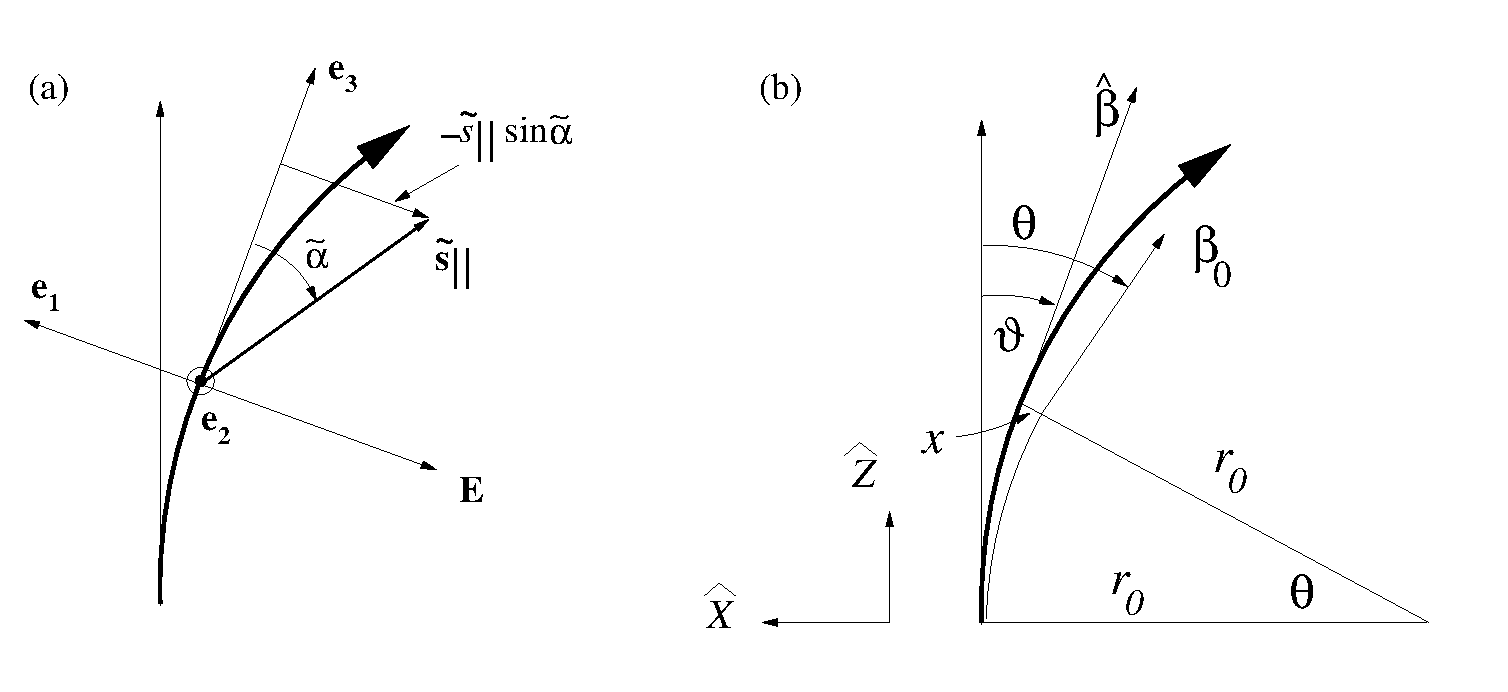
\includegraphics[scale=0.5]{xfig/Precess-reflected.eps}
\caption{\label{fig:Precess}
(a) In the bend plane the
spin vector ${\bf s}$ has precessed through angle
$\tilde \alpha$ away from its nominal direction along the
proton's velocity. (Remember that different particles
have different bend planes.)
(b) Projection of figure~(a) onto the laboratory horizontal
plane. The projected longitudinal axis is shown
coinciding with the laboratory longitudinal axis, even
if this is not exactly valid. $x$ is the deviation of 
the (bold face) particle orbit from the (pale face) design orbit. 
If the bend plane coincides with the design bend plane (as is 
always approximately the case) $\hat{\pmb \beta}_0$ and 
${\bf\hat z}$ are identical. $\theta$ is the reference
particle deviation angle from longitudinal and $\vartheta$
is the tracked particle deviation angle from longitudinal. 
On the average $\theta$ and $\vartheta$ are the same, but
betatron oscillations cause them to differ on a turn by turn
basis, and also to make the instantaneous bend plane not
quite horizontal.}
\end{figure}
%

From the particle tracking one has the laboratory frame
vectors ${\bf r}$, {\bf p}, and hence 
${\bf L}={\bf r}\times {\bf p}$, just past the bend entrance, and
one also has the spin vector ${\bf s}$;
%
\begin{align}
{\bf r} &= r_x{\bf \hat x} + r_y{\bf \hat y} + r_z{\bf \hat z}, \notag\\ 
{\bf p} &= p_x{\bf \hat x} + p_y{\bf \hat y} + p_z{\bf \hat z}, \notag\\ 
{\bf L} &= L_x{\bf \hat x} + L_y{\bf \hat y} + L_z{\bf \hat z}, \notag\\ 
{\bf s} &= s_x{\bf \hat x} + s_y{\bf \hat y} + s_z{\bf \hat z}. 
\label{eq:SpinRot.1}
\end{align}
%
We can establish an orthonormal, right-handed basis triad with axis~3
parallel to ${\bf p}$ and axis~2 parallel to ${\bf -L}$ (where the
negative sign is appropriate for clockwise orbits);
%
\begin{align}
{\bf e_3}
 &= 
  \frac{p_x}{p}\,{\bf \hat x} 
+ \frac{p_y}{p}\,{\bf \hat y} 
+ \frac{p_z}{p}\,{\bf \hat z}, \notag\\
{\bf e_2} &= \frac{{\bf r}\times {\bf p}}{-L}, \notag\\
{\bf e_1} &= {\bf e_2}\times{\bf e_3}.
\label{eq:SpinRot.2}
\end{align}
%
These equations can be re-expressed formally, with all coefficients known, as
%
\begin{align}
{\bf e_1}
 &= 
a_{11}{\bf\hat x}+a_{12}{\bf\hat y}+a_{13}{\bf\hat z}\notag\\
{\bf e_2}
 &= 
a_{21}{\bf\hat x}+a_{22}{\bf\hat y}+a_{23}{\bf\hat z}\notag\\
{\bf e_3}
 &= 
a_{31}{\bf\hat x}+a_{32}{\bf\hat y}+a_{33}{\bf\hat z}.
\label{eq:SpinRot.3}
\end{align}
%
The vector ${\bf s}$ can be expanded as
%
\begin{align}
{\bf s}
 &=
\tilde s_1{\bf e_1} + \tilde s_2{\bf e_2} + \tilde s_3{\bf e_3} \notag\\
 &= \tilde s_1( a_{11}{\bf\hat x}+a_{12}{\bf\hat y}+a_{13}{\bf\hat z}) + \dots \notag\\
 &= (a_{11}\tilde s_1 + a_{21}\tilde s_2 + a_{31}\tilde s_3)\,{\bf\hat x} + \dots.
\label{eq:SpinRot.4}
\end{align}
%
The final relation can be expressed in matrix form as
%
\begin{equation}
\begin{pmatrix} s_x \\ s_y \\ s_z \end{pmatrix}
 =
{\bf R}
\begin{pmatrix} \tilde s_1 \\  \tilde s_2 \\  \tilde s_3 \end{pmatrix},
\label{eq:SpinRot.5}
\end{equation}
%
where ${\bf R}$ is an orthogonal matrix,
%
\begin{equation}
{\bf R}
 =
\begin{pmatrix} a_{11} & a_{21} &  a_{31}  \\  
                a_{12} & a_{22} &  a_{32}  \\  
                a_{13} & a_{23} &  a_{33}  
\end{pmatrix}.
\label{eq:SpinRot.6}
\end{equation}
%
(Aside: the magnitude $|{\rm det}{\bf R}|$ of the determinant of 
${\bf R}$ is necessarily 1, but the actual value is $\pm1$.
This sign correlates with the clockwise/counterclockwise
orbit ambiguity.)

Because ${\bf R}$ is orthogonal, ${\bf R}^{-1}={\bf R}^T$ and  
Eq.~(\ref{eq:SpinRot.5}) can be inverted to give 
%
\begin{equation}
\begin{pmatrix} \tilde s_1 \\  \tilde s_2 \\  \tilde s_3 \end{pmatrix}
 =
\begin{pmatrix} a_{11} & a_{12} &  a_{13}  \\  
                a_{21} & a_{22} &  a_{23}  \\  
                a_{31} & a_{32} &  a_{33}
\end{pmatrix} \,
\begin{pmatrix} s_x \\ s_y \\ s_z \end{pmatrix}.
\label{eq:SpinRot.7}
\end{equation}
%
This yields the spin components in the bend frame. Their propagation
through the bend is described below. At the exit of the bend element
the laboratory-frame components can be worked out using a similar 
formula.

\subsubsection{Non-Bend Elements}
Some elements (especially quadrupoles)
can cause vertical deflections which alter $s_y$.
Being proportional
to transverse displacements these deflections are
very small and can have either polarity.
Nevertheless it is necessary to keep track of their
effects. 

On an element by element basis, when a particle 
has just entered an element that bends (for example) in a
plane rolled counter-clockwise by angle $\phi$ about 
the $z$-axis,
it is first necessary to transform its laboratory frame 
coordinates $(s_x,s_y,s_z)$ into bend frame coordinates
$(\tilde s_x,\tilde s_y,\tilde s_z)$ using
%
\begin{equation}
\begin{pmatrix} \tilde s_x \\ \tilde s_y \\ \tilde s_z \end{pmatrix}
 =
\begin{pmatrix} 
 \cos\phi  & -\sin\phi  &  0 \\
 \sin\phi  &  \cos\phi  &  0 \\
    0      &     0      &  1
\end{pmatrix}
\begin{pmatrix} s_x \\ s_y \\ s_z \end{pmatrix}
\label{eq:SpinPrecess.0p}
\end{equation}
%
(As it stands, this equation is over-simplified since (in the
presence of vertical betatron oscillation) the normal to the
bend plane can have a (tiny) component along the longitudinal
axis. This complication is temporarily being ignored.)
The roll angle $\phi$ has been chosen so that the
element causes pure precession through 
some calculable angle $\widetilde{\Delta\alpha}$ about 
some known axis. With the particle speed known, 
$\widetilde{\Delta\alpha}$ is determined unambiguously by
the (known) magnitude of the angular deflection in the multipole 
element. The plane
of deflection is also available from the particle tracking
through the element.
Expressing the spin precession also by a $3\times3$ matrix, 
and transforming back to the erect laboratory frame,
one obtains the new cartesian components,
%
\begin{equation}
\begin{pmatrix} s_x \\ s_y \\ s_z \end{pmatrix}_{\rm after}
 =
\begin{pmatrix} 
 \cos\phi  &  \sin\phi  &  0 \\
-\sin\phi  &  \cos\phi  &  0 \\
    0      &     0      &  1
\end{pmatrix}
\begin{pmatrix} 
 \cos\widetilde{\Delta\alpha}  &  0  & -\sin\widetilde{\Delta\alpha}  \\
           0                   &  1  &              0                 \\
 \sin\widetilde{\Delta\alpha}  &  0  &  \cos\widetilde{\Delta\alpha}  
\end{pmatrix}
\begin{pmatrix} 
 \cos\phi  & -\sin\phi  &  0 \\
 \sin\phi  &  \cos\phi  &  0 \\
    0      &     0      &  1
\end{pmatrix}
\begin{pmatrix} s_x \\ s_y \\ s_z \end{pmatrix}_{\rm before}
\label{eq:SpinPrecess.0q}
\end{equation}
%
As mentioned earlier, matrix products like these are to be 
explicitly concatenated, outside ETEAPOT, 
with all elements expressed as (rapidly convergent) truncated
expansions in products of (small) angles and 
(small) precession angle $\widetilde{\Delta\alpha}$. 
The resultant matrix (coded into ETEAPOT) differs from the 
identity matrix only by differentially-small, 
rapidly-convergent elements.

\subsection{Spin Evolution Through Mu\~noz-Pavic Bends}
\subsubsection{Analytic Formulas for Spin Precession}
We introduce, at least temporarily, the term 
``Mu\~noz-Pavic Bend'' to characterize a bend
having field index $m=1$, which is the case being treated in our
2D formalism. In this case (and only in this case)
the orbit stays in a single plane. Also,
in this frame any precession of the spin is purely around an 
axis normal to the plane. Obtaining the initial values of the
spin components in this frame was described in the previous section. 

In the bend plane the orbit lies in a single plane.
Superficially this may suggest we are accounting
only for horizontal betatron oscillations and neglecting vertical 
betatron oscillations. In fact, however, the
ETEAPOT treatment accounts for arbitrary betatron and synchrotron
motion by assigning different ``wobbling planes'' to each
individual particle. Even allowing for vertical betatron motion
these frames are all very nearly parallel to the global 
horizontal design frame of the ring.
For the 2D evolution through electric bend elements 
in ETEAPOT, any betatron oscillations actually present for
a particular particle are folded into the determination of
its particle-specific orbit plane, and the initial coordinates in 
this plane.

As shown in Figure~\ref{fig:Precess}, the initial spin vector is
%
\begin{equation}
{\bf \tilde s}
 = 
 -\tilde s_{\parallel}\sin\tilde\alpha\,{\bf\hat x}
 +\tilde s_y{\bf\hat y} 
 +\tilde s_{\parallel}\cos\tilde\alpha\,{\bf\hat z}.
\label{eq:SpinPrecess.9}
\end{equation}
%
Here $\tilde s_y{\bf\hat y}$ is the out-of-plane component of ${\bf \tilde s}$,
$\tilde s_{\parallel}$ is the magnitude of the in-plane projection of ${\bf \tilde s}$, 
and $\tilde\alpha$
is the angle between the projection of ${\bf \tilde s}$ onto the plane
and the tangent vector to the orbit.

Jackson's\cite{Jackson} Eq.~(11.171) gives the rate of change 
in an electric field ${\bf E}$, of the longitudinal spin component as
%
\begin{equation}
\frac{d}{dt}\,
({\bf\hat\beta\cdot s})
 =
-\frac{e}{m_pc}\,
({\bf s_{\perp,J}\cdot E})
\bigg(
\frac{g\beta}{2} - \frac{1}{\beta}
\bigg).
\label{eq:SpinPrecess.1}
\end{equation}
%
(Note that Jackson's ${\bf s}_{\perp,J}$ is the component perpendicular
to the tangent to the orbit \emph{not} to the orbit plane.)
Substituting from Eq.~(\ref{eq:SpinPrecess.9}) the 
equation becomes
%
\begin{equation}
\frac{d}{dt}\,
(\tilde s_{\parallel}\cos\tilde\alpha)
 =
-\frac{e}{m_pc}\,
(\tilde s_{\parallel}\sin\tilde\alpha\,E)\,
\bigg(
\frac{g\beta}{2} - \frac{1}{\beta}
\bigg).
\label{eq:SpinPrecess.1mp}
\end{equation}
%
With the orbit confined to a plane,
any precession occurs about the normal to the plane,
conserving $\tilde s_y$. Since the magnitude of ${\bf \tilde s}$ is
conserved it follows that the magnitude $\tilde s_{\parallel}$
is also conserved. This allows $\tilde s_{\parallel}$ to be 
treated as constant in Eq.~(\ref{eq:SpinPrecess.1mp}).
Then Eq.~(\ref{eq:SpinPrecess.1mp}) reduces to
%
\begin{equation}
\frac{d\tilde\alpha}{dt}\,
 =
\frac{eE}{m_pc}\,
\bigg(
\frac{g\beta}{2} - \frac{1}{\beta}
\bigg).
\label{eq:SpinPrecess.2}
\end{equation}
%
This is undoubtedly a fairly good approximate equation in any
more-or-less constant electric field, but it is \emph{exact only for
the $m=1$ Keplerian electric field}, which is the only field
in which arbitrary orbits stay in a fixed plane.  In fact, the
derivation is not quite valid even for our $m=1$ case.  Though
the design orbit is circular, the betatron orbits are slightly
elliptic. This violates our assumption that orbit and electric 
field are orthogonal. Neglecting this amounts to dropping a 
term from the RHS of Eq.~(\ref{eq:SpinPrecess.1}) that is
down by four orders of magnitude. Furthermore this term would 
average to zero except for a possible non-zero
commutation precession which would be expected to be down by 
another four orders of magnitude.

Meanwhile the velocity vector itself has precessed by angle 
$\vartheta$ relative to a direction fixed in the laboratory. 
Note that this angle $\vartheta$, the angle of the 
individual particle's orbit is approximately, but not exactly 
equal to the angle $\theta$ of the design orbit.

In the ETEAPOT treatment each particle in an electric bend
element evolves in its own plane. 
${\bf \tilde s}_{\parallel}$ is the component in this plane of the total
spin vector. At every entrance to an electic bend ${\bf \tilde s}_{\parallel}$
has to be calculated from the known laboratory frame description
of ${\bf s}$, which also has to be updated as the particle exits
the bend. (Ideally, in an EDM storage ring experiment any out-of-plane
component of ${\bf s}$ would be evidence of non-vanishing electric dipole
moment.) 

The precession rate of $\vartheta$ is governed by the equation
%
\begin{equation}
\frac{d\vartheta}{dt}
 =
\frac{d}{dt}\,\bigg(\frac{s}{r}\bigg)
 =
\frac{eE}{p}.
\label{eq:SpinPrecess.3}
\end{equation}
%
where the curvature is $1/r=eE/(v p)$ and
(just in this equation) $s$ temporarily stands for arc
length along the orbit. Dividing Eq.~(\ref{eq:SpinPrecess.2})
by Eq.~(\ref{eq:SpinPrecess.3}) and using $pc=m_pc^2\gamma\beta$,
%
\begin{equation}
\boxed{
\frac{d\tilde\alpha}{d\theta}
 =
\bigg(
\frac{g}{2} - 1
\bigg)\,\gamma
 -\frac{g/2}{\gamma}
.
\label{eq:SpinPrecess.4}
}
\end{equation}
%
In this step we have also surrepticiously made the
replacement $\vartheta\rightarrow\theta$. Even though
these angles are not the same, over arbitrarily long
times they advance at the same rate. In any case the
error in equating $\vartheta$ to $\theta$
becomes progressively more valid in the fine-slicing 
limit, as the orbit is more nearly approximated by
straight line segments.
Explicitly the bend frame precession advance is the sum of two
definite integrals
%
\begin{equation}
\widetilde{\Delta\alpha}
 =
\bigg(
\frac{g}{2} - 1
\bigg)\,I_\gamma
 -
\frac{g}{2}I_{\gamma i},
\label{eq:SpinPrecess.4p}
\end{equation}
%
where 
%
\begin{equation}
I_\gamma = \int_0^{\theta}\,\gamma(\theta') d\theta',
\quad\hbox{and}\quad
I_{\gamma i} = \int_0^{\theta}\,\frac{d\theta'}{\gamma(\theta')}.
\label{eq:SpinPrecess.4q}
\end{equation}
%
To account for fringe fields two more
terms, $\widetilde{\Delta\alpha}^{\rm FF,in}$ and 
$\widetilde{\Delta\alpha}^{\rm FF,out}$, will later be added directly 
to the right hand side of Eq.~(\ref{eq:SpinPrecess.4p}).

\subsubsection{Non-Perturbative Evaluation of the Spin Precession}
Eq.~(\ref{eq:SpinPrecess.4}) is susceptible to solution
by an approach just like that used in the time of flight
determination. 
The main step is to express $\gamma$ as a function of $\theta'$;
%
\begin{align}
\gamma(\theta')
 &=
\frac{\mathcal{E}/e}{m_pc^2/e}
 -
\frac{E_0r_0}{m_pc^2/e}\,
\Big(
\xi_{\rm co}
 + 
(\xi_{\rm in}-\xi_{\rm co})\,\cos Q\theta'
 + 
\frac{\xi'_{\rm in}}{Q}\,\sin Q\theta'
\Big) \notag \\
 &\equiv
a + b\cos{Q\theta'} + c\sin{Q\theta'}.
\label{eq:SeriesSpinPrecess.1}
\end{align}
%
After this replacement, $\theta'$ is the only variable factor on 
the RHS of Eq.~(\ref{eq:SpinPrecess.4}). All of the integrals can
be evaluated in closed form. The more complicated integral
is given by
%
\begin{equation}
I_{\gamma i}(\theta)Q
 = 
Q\int_0^{\theta}\,\frac{d\theta'}{a + b\cos{Q\theta'} + c\sin{Q\theta'}}.
\label{eq:SeriesSpinPrecess.2}
\end{equation}
%
A prescription for evaluating such integrals is given, for example,
in Dwight\cite{Dwight}, formula 456.2. Define 
$r=\sqrt{b^2+c^2}$, $\sin\psi=b/r$, and $\cos\psi=\pm c/r$.
(In the code one must use $\psi=$arctan2($b,\pm c$) to obtain $\psi$,
to handle the $r=0$ possibility.) The reason for the introduction of
th $\pm$ option is explained below; until then assume the
$+$ option has been chosen. The indefinite integral is transformed to 
%
\begin{equation}
\int\,\frac{d(Q\theta' + \psi)}{a + r\sin(Q\theta' + \psi)}.
\label{eq:SeriesSpinPrecess.3}
\end{equation}
%
Then, defining $x'=Q\theta' + \psi$, one obtains 
%
\begin{equation}
I_{\gamma i}(\theta)Q
 = 
\int_{ \psi}^{ \psi+Q\theta}\,\frac{dx'}{a + r\sin x'}.
\label{eq:SeriesSpinPrecess.4}
\end{equation}
%
The form of this integral, as given in Dwight 436.00, depends
on the relative magnitudes or $a$ and $r$. In our storage ring
application the oscillating part of $\gamma$ is always miniscule
compared to its nominal value. As a result $|a| >> |r|$ and the
result is
%
\begin{equation}
I_{\gamma i}(\theta)Q
 = 
\bigg[
\frac{2}{\sqrt{a^2-r^2}}\,
{\rm arctan}
\Big(
\frac{a\tan{x'/2} + r}{\sqrt{a^2-r^2}}
\Big)
\bigg]_{ \psi}^{\psi+Q\theta}.
\label{eq:SeriesSpinPrecess.5}
\end{equation}
%
In this case the denominator of the arctan argument cannot vanish.
Also, practical bend element bend angles satisfy $\theta<<\pi/2$
and the arctan evaluation is unambiguous. For realistically short
bend elements the $\widetilde{\Delta\alpha}$ increment cannot exceed a
few percent. 

Another hazard to be faced is the possibility for the upper and
lower limits in Eq.~(\ref{eq:SeriesSpinPrecess.5}) to be
on opposite sides of a discontinuity in the arctan function.
This was the motivation for introducing the $\pm$ option.
Switching the initial choice from $+$ to $-$ is equivalent to switching
the sign of $\psi$. The $\psi=0$ possibility can be ignored since,
in that case, there would be no possibility of upper and lower limits 
straddling the discontinuity. Switching the sign of $\psi$ therefore
gives two independent choices of upper and lower limits in 
Eq.~(\ref{eq:SeriesSpinPrecess.5}) and, therefore, two evaluations
of the definite integral, of which at most one is incorrect. It
is not hard to decide which determination to discard. It has already
been stated that the $\widetilde{\Delta\alpha}$ increment cannot exceed a
few percent. Numerically this test has proved to be sufficient in
numerous cases. But, as a further check, a perturbative evaluation,
not subject to the arc tangent ambiguity, is described in the next
section. The perturbative evaluation always agrees with the (correct)
non-perturbative evaluation to 1/10 percent accuracy.

It has been stated that practical bend elements bend at most through
a few degrees. The ETEAPOT code has no such constraint, however. The
{\tt sxf} file could, for example, represent a single inverse square
law electric field of total bend angle arbitrarily larger than $2\pi$.
Though impractical for a storage ring, the resulting evolution can
be (and has been) checked against celestial mechanics evaluations, 
such as those of Mu\~noz. The precautions described in the previous
paragraph have to be altered for this case.

It is important not to apply any magnitude test to 
the accumulated precession angle $\tilde\alpha$, because its
magnitude can become arbitrarily large over long times.

\subsubsection{Perturbative Treatment Relative to the Magic Condition}
In an EDM storage ring, the design $\gamma$ value
is set equal to the ``magic'' value $\gamma_0$. This
suggests using the difference $\gamma-\gamma_0$ as independent
variable for purposes of energy expansions. In practice this
is likely to lead to confusion when, intentionally or 
unintentionally, the design value $\gamma_D$ is not quite
equal to $\gamma_0$. If a ``magic'' (in its physics sense) 
value is hard-coded then it becomes ``magic'' (in the computer
science sense); which is something to be avoided. To avoid
this we define, instead, with ``D'' standing for ``design'',
%
\begin{equation}
\Delta\gamma
 = 
\gamma - \gamma_D,
\label{eq:SpinPrecess.1m}
\end{equation}
%
planning, usually, to identify $\gamma_D$ with $\gamma_0$. 
Any particular particle being tracked will typically
have a $\gamma$ value different from both the magic value $\gamma_0$
and the design value $\gamma_D$.
With $\gamma_D=\gamma_0$, 
one can check that $d\tilde\alpha/d\theta$ vanishes at the magic 
condition $\gamma=\gamma_0$; 
%
\begin{equation}
\Big(\frac{g}{2}-1\Big)\,\gamma_D - \frac{g/2}{\gamma_D}
 =
0.
\label{eq:ChromaticDev.1}
\end{equation}
%
where $a\equiv G = 1.7928474$, $g=2G+2 = 5.5856948$. The ``magic'' relativistic
factor is $\gamma_0=\sqrt{g/(g-2)}=1.2481073$.
Exploiting this relation, substituting from Eq.~(\ref{eq:SpinPrecess.1m}),
and expanding in powers of $\Delta\gamma$,
%
\begin{align}
\frac{d\tilde\alpha}{d\theta}
 &=
\Big(\frac{g}{2}-1\Big)\,(\gamma_d + \Delta\gamma)
 -
\frac{g/(2\gamma_d)}{1+\delta\gamma/\gamma_d}          \notag \\
 &=
\Big(\frac{g}{2}-1\Big)\,\Delta\gamma
 +
\frac{g}{2\gamma_D}
\Big(
\frac{\Delta\gamma}{\gamma_D}
 - \frac{\Delta\gamma^2}{\gamma^2_D}
 + \frac{\Delta\gamma^3}{\gamma^3_D}
 - \dots
\Big).
\label{eq:ChromaticDev.2}
\end{align}
%
The infinite series in Eq.~(\ref{eq:ChromaticDev.2})
would be slowly convergent except for the fact that,
typically, in an storage ring, $\Delta\gamma/\gamma_0<10^{-3}$.
So the expansion can be applied to an arbitrary accelerator
and not just a frozen spin accelerator. Furthermore, at little
computational cost, the series can be truncated with no numerical
test nor defined tolerance, just by retaining a conservatively large 
number of terms.

From initial 
displacements $(x_{\rm in},x'_{\rm in})$ one introduces intermediate variables,
%
\begin{equation}
\xi_{\rm in} = \frac{x_{\rm in}}{r_0+x_{\rm in}},
\quad
\xi_{\rm in}' = \frac{r^2_0x_{\rm in}'}{(r_0+x_{\rm in})^2}.
\label{eq:SpinPrecess.5}
\end{equation}
%
In terms of these variables, neglecting the $\xi_{\rm co}$ offset,
evolution through a Mu\~noz-Pavic bend from $\theta=0$ 
to $\theta$ can be approximated by
%
\begin{align}
\frac{\Delta\gamma(\theta)}{\gamma_D}
 &=
\frac{\mathcal{E}}{m_pc^2\gamma_D}
 -1
 - \frac{eE_0r_0}{m_pc^2\gamma_D}\,
\Big(
\cos(Q\theta)\,\xi_{\rm in}
 + 
\frac{\sin(Q\theta)}{Q}\,\xi'_{\rm in}
\Big)                         \notag\\
 &=
\frac{\Delta\gamma}{\gamma_D}
 +
\frac{eE_0r_0\xi_{\rm in}}{m_pc^2\gamma_D}
 - \frac{eE_0r_0}{m_pc^2\gamma_D}\,
\Big(
\cos(Q\theta)\,\xi_{\rm in}
 + 
\frac{\sin(Q\theta)}{Q}\,\xi'_{\rm in}
\Big) 
\label{eq:SpinPrecess.6}
\end{align}
%
Substituting from Eq.~(\ref{eq:SpinPrecess.5}) 
into Eq.~(\ref{eq:ChromaticDev.2}) one finds,
to a lowest approximation, 
and continuing to assume $\gamma_D=\gamma_0$,
%
\begin{align}
\frac{d\tilde\alpha}{d\theta}
 &\approx
\Big(\frac{g}{2}-1\Big)\,\Delta\gamma
 +
\frac{g}{2\gamma_D}\,
\Big(
\frac{\Delta\gamma}{\gamma_D}
\Big)              \notag \\
 &=
\Big(\frac{g}{2}-1\Big)\,\Delta\gamma
 +
\frac{g}{2\gamma_D}\,
\bigg(
\frac{\Delta\gamma}{\gamma_D}
 +
\frac{eE_0r_0\xi_{\rm in}}{m_pc^2\gamma_D}
 - \frac{eE_0r_0}{m_pc^2\gamma_D}\,
\Big(
\cos(Q\theta)\,\xi_{\rm in}
 + 
\frac{\sin(Q\theta)}{Q}\,\xi'_{\rm in}
\Big)
\bigg)  \notag \\
 &=
\Big(\frac{g}{2}-1\Big)\,\Delta\gamma
 +
\frac{g}{2\gamma_D}\,
\bigg(
\frac{\Delta\gamma}{\gamma_D}
+ \frac{eE_0r_0}{m_pc^2\gamma_D}\,
\Big(
\big(1-\cos(Q\theta)\big)\,\xi_{\rm in}
 - 
\frac{\sin(Q\theta)}{Q}\,\xi'_{\rm in}
\Big)
\bigg).         
\label{eq:SpinPrecess.7}
\end{align}
%
This can be trivially integrated to give $\widetilde{\Delta\alpha}$. 
The total energy $\mathcal{E}$,
is a constant of the motion (not counting RF cavities).
If needed, higher order terms can be included
similarly.

The phase advance over any single Mu\~noz-Pavic bend will
normally be very small compared to $2\pi$ and the
oscillating factor can have either sign. In fact the phase
advances may sometimes be sufficiently small across individual
bends to legitimize approximating $\cos Q\theta\approx1$ and 
$\sin(Q\theta)\approx Q\theta$ to give a quick ``ball park''
estimate of the spin precession.  

The way vertical betatron oscillations are treated
in ETEAPOT, is to regard the Mu\~noz-Pavic plane
as being slightly tilted. This is why the result
in Eq.~(\ref{eq:SpinPrecess.7}) has been expressed
as $\widetilde{\Delta\alpha}$. As explained previously,
small spin orientation corrections are required
at entrance to and exit from bend elements, to consistently
integrate the 3D and 2D descriptions. 

\subsection{Spin Evolution Through Fringe Fields}
So far in ETEAPOT, as a particle enters or exits a bend element, 
its potential
energy has been treated as changing discontinuously with 
its kinetic energy changing correspondingly. We now have
to treat this region more carefully. Instead of treating
the potential as discontinuous, we now assume the change 
occurs over a longitudinal distance $\Delta z^{\rm FF}$ which, for 
estimation purposes, we take equal to the separation 
distance (symbol $gap$) between the electrodes; $\Delta z=gap$. 
(For the ``protonium'' model introduced later, the drift lengths
are taken to be almost zero and fringe field spin precession
is negligible.)
The fringe field region is assumed to be short enough to
be treated as ``thin''. That is, 
any change in the particle's radial offset
occuring in range $\Delta z$ is to be neglected and the
integrated deflection applied at the center (i.e. the
edge of the bend). As a result 
the curve $x(z)$ is continuous, but its slope $dx/dz$ is 
discontinuous. Entrance transitions 
from outside a bend to inside are described first.

Inside the bending element
the increase in potential energy from orbit
centerline to radial position $x$ is $e\Delta V(x)$. 
As synchroton oscillations move the particle radially in
and out, the sign of $\Delta V(x)$, just inside the
bend edge oscillates between negative and positive values, 
and the sign of the deviation from the magic velocity 
oscillates correspondingly. This will tend to
average away the spin run-out occurring in the fringe field
region over times long compared to
the synchrotron period. In the long run it is the deviation 
from zero of this average that has to be determined. This can be
by pure numerical tracking or theoretically or, 
most likely, by a theoretical averaging based on numerical
tracking data.

Once one is able to determine the spin decoherence the task will
shift to designing sextupole distributions capable of increasing
the spin coherence time SCT. Our approach will be to study
the effectiveness of such schemes before attempting to improve
the precision of our fringe field treatment.

The deflection angle $\theta^{(FF)}$ of the design orbit in
the fringe field at one such edge is approximately
%
\begin{equation}
\theta^{(FF)}
 \approx
\frac{1}{2}\,
\frac{\Delta z^{\rm FF}}{r_0}
\quad
\Big(
\overset{\rm e.g.}{\ =\ }
0.5\times0.03/40
 =
0.375\times10^{-3}
\Big);
\label{eq:FF.1}
\end{equation}
%
this is half of the deflection occurring in advancing a
distance $gap$ in the interior of the bend. (The angle $\theta^{(FF)}$ 
is implicitly assumed to be positive, irrespective of whether the
orbit is clockwise or counter-clockwise.)
Consider a particle approaching the fringe field region
at radial displacement $x$. At the longitudinal center of the fringe field
region the kinetic energy of this particle deviates
from its ``proper'' (i.e. fully-inside value at radial displacement $x$)
by the amount
%
\begin{equation}
\Delta\gamma^{(FF)}(x)
 \approx
\frac{1}{2}\,
\frac{\Delta V(x)}{m_pc^2/e}
 \approx
\frac{1}{2}\,
\frac{E\,x}{m_pc^2/e},
\label{eq:FF.2}
\end{equation}
%
where $\Delta V_{\rm tot}$ is the total voltage 
increase from inner electrode to outer electrode.
(The electric 
field points radially inward in order for
positive particles to bend toward negative $x$
but, by convention, $E$ is positive.)
Here, for simplicity, we are neglecting the
fact that the actual electric field will have
more complicated $x$-dependence depending,
for example, on the value of the field index $m$. 
Our assumed fringe field spatial dependence is also 
simplistic.

According to Eq.~(\ref{eq:ChromaticDev.2}) the
leading effect of passage through a bend region
with $\gamma$ deviation from magic $\Delta\gamma$,
is a rate of change of spin angle $\alpha$ per
unit deflection angle $\theta$ given by
%
\begin{equation}
\frac{d\alpha}{d\theta}
 \approx
\bigg(\frac{g}{2} - 1 + \frac{g/2}{\gamma_0^2}\bigg)\,\Delta\gamma
\quad
\Big( \overset{\rm for\ proton}{\quad=\quad}
3.586\,\Delta\gamma.
\Big)
\label{eq:FFsinglePass.1}
\end{equation}
%
Combining equations, the excess angular advance occurring
while entering the bend at displacement $x$ is 
%
\begin{equation}
\boxed{
\widetilde{\Delta\alpha}^{\rm FF}
 =
+\bigg(\frac{g}{2} - 1 + \frac{g/2}{\gamma_0^2}\bigg)\,
\frac{1}{2}\,
\frac{E\,x}{m_pc^2/e}\,
\frac{1}{2}\,
\frac{\Delta z^{\rm FF}}{r_0}.
\label{eq:FFsinglePass.1p}
}
\end{equation}
%
({\bf Aside:} it may be appropriate to keep another term in
expansion~(\ref{eq:FFsinglePass.1}) in order to include
the effect that dispersion introduces a correlation between
$\gamma$ and $x$ which, after averaging, leaves a finite
precession, even if $<x>$ vanishes
in Eq.~(\ref{eq:FFsinglePass.1p}) .)

In our initial treatment of this edge effect we are assuming
this precession lies in exactly the same plane as the
orbit plane of the particle in the bend element, justifying
the notation $\widetilde{\Delta\alpha}^{\rm FF}$
Entrance (and, later, exit) values can simply be added to the
main precession through the bend element.
Meanwhile, in the fringe field region the advance of the tangent 
to the orbit is $\theta^{(FF)}$ as given by Eq.~(\ref{eq:FF.1}).
The + sign on the rhs of Eq.~(\ref{eq:FFsinglePass.1p}) 
reflects the fact that,
for a particle displaced radially outward, the particle momentum
is completing some of its rotation in the fringe field where 
its magnitude is more positive than in the bend interior.

Though the fringe field precession occurs continuously
over the range $gap$ it is applied discontinuously at
the bend edge. This is consistent with our hard edge treatment
of the particle's momentum evolution.
Because $\widetilde{\alpha}$ is measured relative to the orbit direction,
Eq.~(\ref{eq:FFsinglePass.1p}) gives the spin angle precession
over and above the advance of the tangent to the orbit.

The fact that spin and momentum angular advances do not 
match has come about because the particle has bent appreciably 
while its speed deviates from the magic value. On exiting the 
bend element the particle also bends appreciably while its 
$\gamma$ deviation is given by the same formula~(\ref{eq:FF.2}).
Eq.~(\ref{eq:FFsinglePass.1p}) therefore applies to both entrance 
and exit. Unfortunately this means that excess input precession and 
excess output
precession combine constructively rather than tending to cancel
(as edge focusing sometimes does.)

The largest magnitude $\Delta\gamma^{(FF)}$ can have is
%
\begin{equation}
|\Delta\gamma^{(FF)}_{\rm max}|
 =
\frac{1}{4}\,
\frac{E\,gap}{m_pc^2/e}
\quad
\Big(
\overset{\rm e.g.}{\ =\ }
\frac{1}{4}\,
\frac{(10.5\times10^6)\times0.03}{0.938\times10^9}\,
 =
0.84\times10^{-4}.
\Big)
\label{eq:FF.3m}
\end{equation}
%
For a particle with magic velocity skimming the outer electrode,
where the effect is maximum,
the angular runout is given by 
%
\begin{align}
|\Delta\alpha^{(FF)}_{\rm max}|
 &\approx
\bigg(\frac{g}{2} - 1 + \frac{g/2}{\gamma_0^2}\bigg)\,
\Delta\gamma_{\rm max}\,
\Delta\theta^{(FF)}         \notag\\
 &=
3.586
\times 
(0.84\times10^{-4})
\times
(0.375\times10^{-3})      \notag\\
 &=                      
1.13\times10^{-7}\,{\rm radians/edge}.
\label{eq:FFsinglePass.2}
\end{align}
%
With perhaps 50 edges in the lattice, and revolution frequency of 
about 1\,MHz, the maximum spin runout will be about one
revolution per second. This vastly exaggerates the spin
decoherence, of course, because it does not account for
the averaging effect of synchrotron oscillations.
A challenge for lattice design is
to perfect the synchrotron oscillation averaging to zero. 

\subsection{Spin Evolution Through Thin Elements}
In ETEAPOT the only ``thick'' elements are bends. Spin
evolution through them has already been discussed.
All other elements are treated as thin element kicks. 
Rearranging
Eq.~(\ref{eq:FFsinglePass.1}) produces, for spin evolution
through a thin element,
%
\begin{equation}
\boxed{
|\widetilde{\Delta\alpha}|
 \approx
\bigg(\frac{g}{2} - 1 + \frac{g/2}{\gamma_0^2}\bigg)\,
\Delta\gamma\,
\widetilde{\Delta\theta}
\label{eq:ThinEl.1m}
}
\end{equation}
%
where $\widetilde{\Delta\theta}$ is positive by definition 
and $\widetilde{\Delta\alpha}$ is the angular deviation
of the bend plane spin coordinate relative to the orbit.
The absolute value sign in this equation eventually has
to be removed; it is included here so that the discussion
of signs can be deferred. In paraxial approximation,
for a particle with transverse position $(x,y)$, the 
magnitude of the (not necessarily horizontal) angular deviation 
$\widetilde{\Delta\theta}$ in a quadrupole of strength $q$
is given by
%
\begin{equation}
\widetilde{\Delta\theta} = |q|\sqrt{x^2+y^2},
\label{eq:ThinEl.1p}
\end{equation}
%
where $q$ is the inverse focal length of the quadrupole.
(The magnitude of the angular deflections in sextupoles and 
higher order multipoles are also functions only of the
combination $\sqrt{x^2+y^2}$).

A significant complication concerns the sign of the 
$\widetilde{\Delta\alpha}$. For a 
\emph{horizontally focusing or defocusing quadrupole} 
there is no ambiguity, since the bend plane
in the quadrupole is the same as the overall (horizontal)
lattice design plane. In this case, with $y=0$,
Eq.~(\ref{eq:ThinEl.1m}) can be made more explicit;
%
\begin{equation}
\widetilde{\Delta\alpha}_h
 \approx
\bigg(\frac{g}{2} - 1 + \frac{g/2}{\gamma_0^2}\bigg)\,
\Delta\gamma\,
q\,x.
\label{eq:ThinEl.1q}
\end{equation}
%
where, by convention, a horizontal \emph{focusing} quad has $q>0$. 
The sign in Eq.~(\ref{eq:ThinEl.1q}) reflects the fact that, for 
$x>0$ and $q>0$, the quadrupole ``helps'' by 
bending the momentum in the same sense as the bending elements.
This formula makes it clear that reversing the sign of $q$
reverses the sign of $\widetilde{\Delta\alpha}$.

For obtaining the proper sign for vertically
focusing quadrupoles it is necessary to handle consistently
the transformation from laboratory to bend frame spin
coordinates, which is why the sign issue has been deferred until
after discussing this transformation.

Most of the elements in a storage ring cause
spin precession which approximately conserves the
vertical component of spin $s_y{\bf\hat y}$. The leading
exceptions to this in a proton EDM storage rings are the
vertically focusing or defocusing quadrupoles  
present in the lattice to keep $\beta_x$ magnageably small. 
Particles having non-vanishing vertical betatron amplitude are
deflected vertically which causes $s_y{\bf\hat y}$ to
precess. (As an aside it can be mentioned that there is
a very strong tendency for this precession to cancel
in subsequent quadrupoles and, therefore, probably not
contribute significantly to spin decoherence. Nevertheless
it is important for the precession to be modeled
correctly.)
All quadrupoles and sextupoles in the lattice
cause similar precession to at least some degree. 

The planes of deflection for particles incident on a
quadrupole are shown in Figure~\ref{fig:QuadRotatPlanes}.
In a perfect multipole field the magnitude of the 
total deflection angle
is constant on a contour of fixed radius (i.e. a circle
centered on the origin.) For a particle incident at 
$(x_0,y_0)$ the equation of the line of intersection
of the deflection plane with the transverse plane is
%
\begin{equation}
y = y_0 - \frac{y_0}{x_0}\,(y-y_0),
\label{eq:ThinEl.2}
\end{equation}
%
As shown if the figure, the roll-angle of the deflection plane
(with counter-clockwise roll taken as positive)
is $\phi=\tan^{-1}(y_0/x_0)$,
irrespective of quadrant and whether the quadrupole is
focusing or defocusing. However the inverse tangent function
is, itself, multiple valued. To make it single valued one can
determine $\phi$ using
%
\begin{equation}
\phi={\rm arctan2}(qy_0,qx_0).
\label{eq:ThinEl.3}
\end{equation}
%
Along with Eq.~(\ref{eq:ThinEl.1m}), this establishes
both the sign and magnitude of $\widetilde{\Delta\alpha}$,
while preserving the sign reversal when the sign of $q$ reverses.
This should be checked numerically in all quadrants.
%
\begin{figure}[h]
\centering
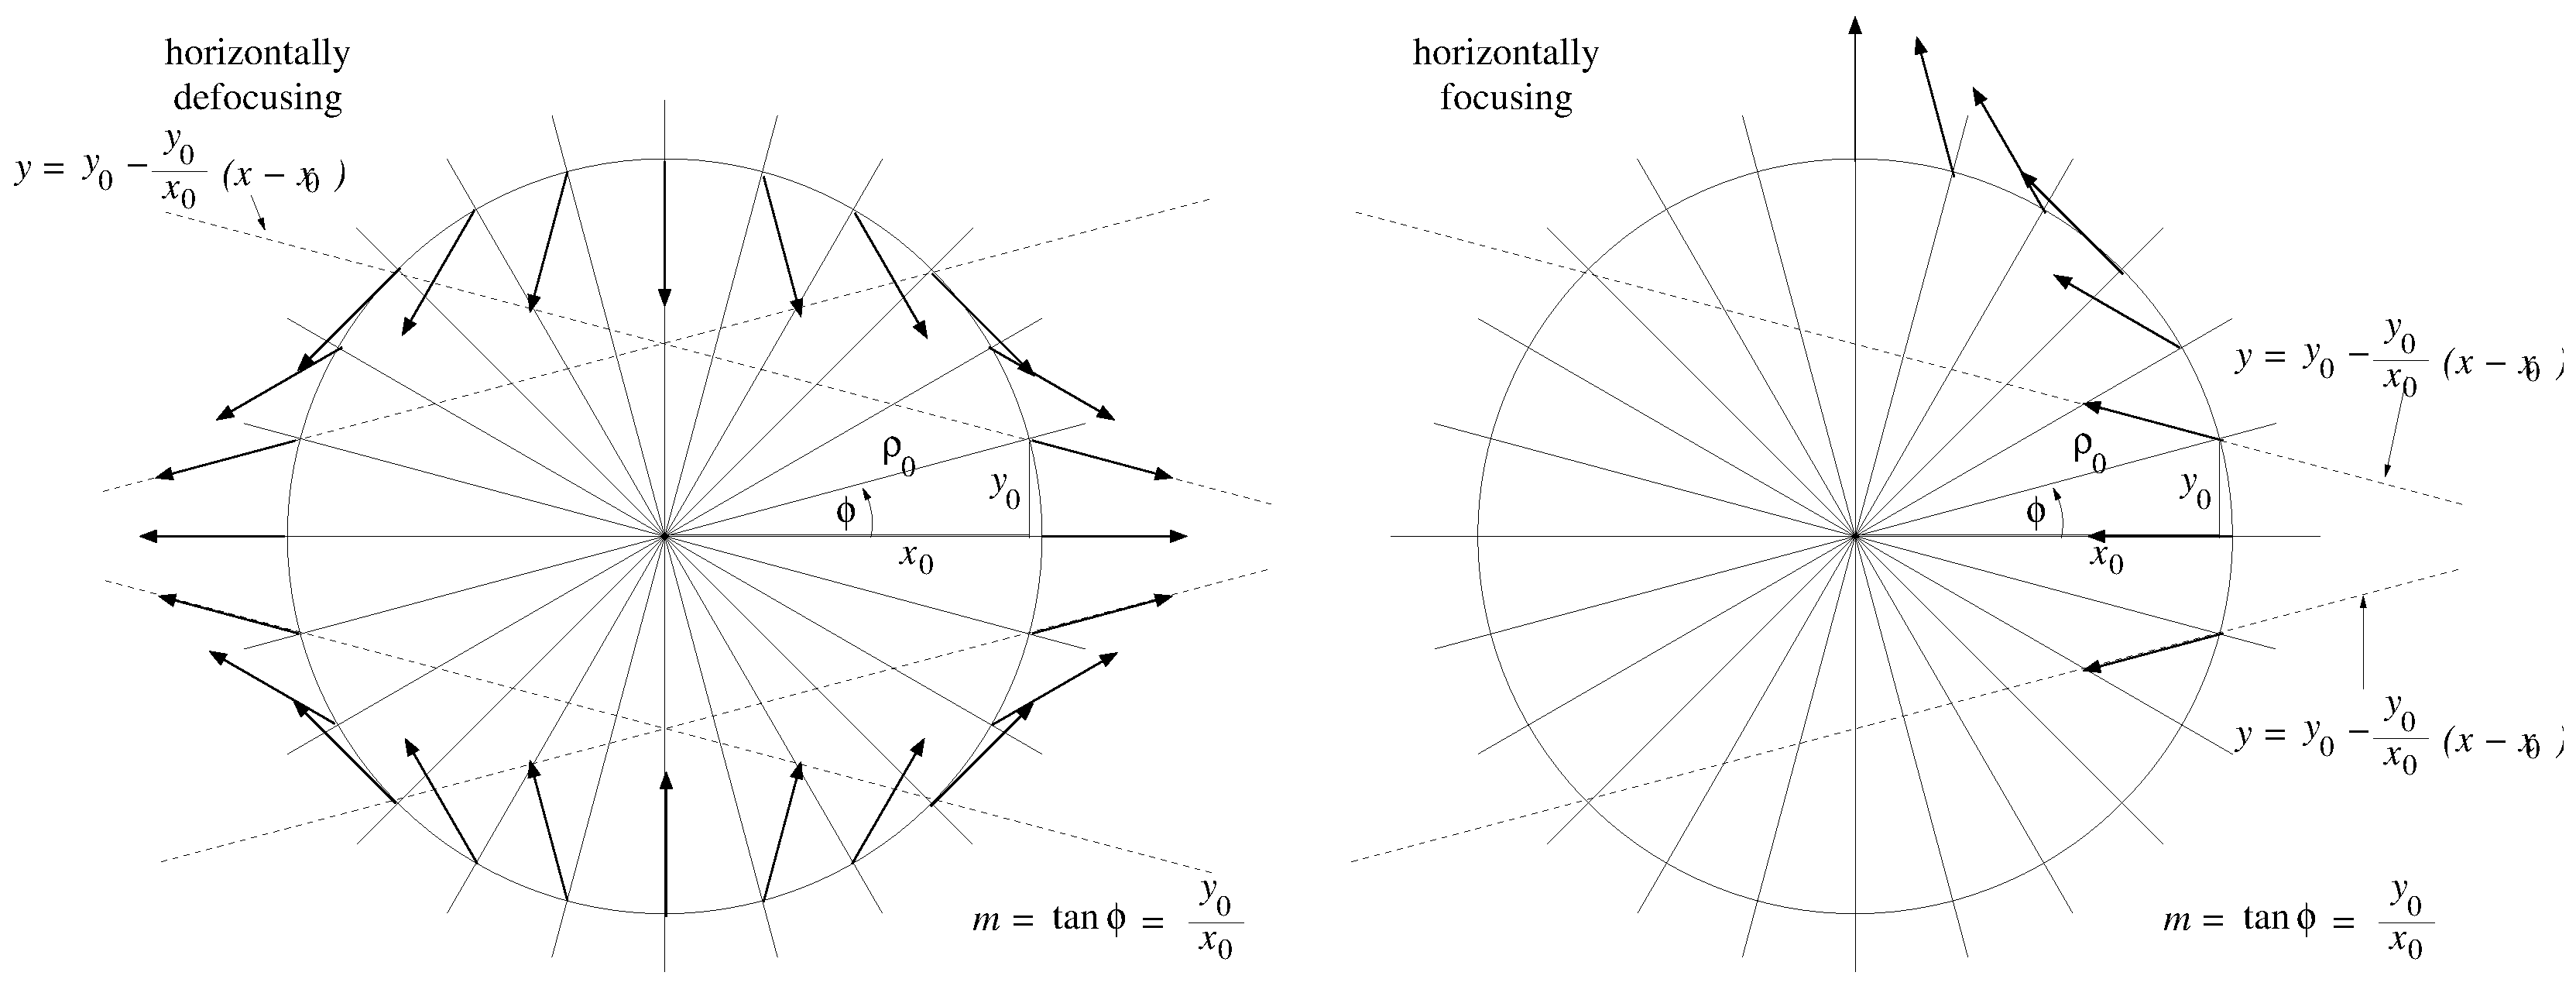
\includegraphics[scale=0.26]{xfig/QuadRotatPlanes.eps}
\caption{\label{fig:QuadRotatPlanes}The broken lines
shows the deflection planes for particle with
dispacements $x_0,y_0$ in various quadrants, incident 
on an erect quadrupole.  The roll-angle of the deflection plane
(with counter-clockwise roll taken as positive)
is $\phi=\tan^{-1}(y_0/x_0)$ irrespective of quadrant,
and irrespective of whether the quadrupole is
focusing or defocusing.}
\end{figure}
%
Substitution into Eq.~(\ref{eq:SpinPrecess.0q}) and
defining $\rho_0=\sqrt{x_0^2+y_0^2}$, produces
%
\begin{equation}
\begin{pmatrix} s''_x \\ s''_y \\ s''_z \end{pmatrix}
 =
\begin{pmatrix} 
  \cos\phi  & -\sin\phi &  0 \\
  \sin\phi  &  \cos\phi &  0 \\
    0       &     0     &  1
\end{pmatrix}
\begin{pmatrix} 
 \cos\widetilde{\Delta\alpha}  &  0  & -\sin\widetilde{\Delta\alpha}  \\
           0                   &  1  &              0                 \\
 \sin\widetilde{\Delta\alpha}  &  0  &  \cos\widetilde{\Delta\alpha}  
\end{pmatrix}
\begin{pmatrix} 
  \cos\phi &  \sin\phi  &  0 \\
 -\sin\phi &  \cos\phi  &  0 \\
    0      &     0      &  1
\end{pmatrix}
\begin{pmatrix} s_x \\ s_y \\ s_z \end{pmatrix}
\label{eq:ThinEl.4}
\end{equation}
%
It is appropriate, to improve numerical precision, to 
break the central matrix into two terms, ${\bf I}+{\pmb\Delta}$
where ${\bf I}$ is the identity matrix and ${\pmb\Delta}$ is a
small deviation. Then, since ${\bf I}$ commutes with the outer
matrices, and their product is ${\bf I}$, the final result is
equal to ${\bf I}$ plus a small deviation. The matrix product is
%
\begin{align}
&\begin{pmatrix} 
  \cos\phi  & -\sin\phi &  0 \\
  \sin\phi  &  \cos\phi &  0 \\
    0       &     0     &  1
\end{pmatrix} 
\Bigg(
\begin{pmatrix} 
  1  &  0  &  0  \\
  0  &  1  &  0  \\
  0  &  0  &  1  
\end{pmatrix}
 +
 2\sin(\widetilde{\Delta\alpha}/2)
\begin{pmatrix} 
 -\sin\widetilde{\Delta\alpha}/2 &  0  & -\cos\widetilde{\Delta\alpha}/2  \\
             0                   &  1  &              0                   \\
  \cos\widetilde{\Delta\alpha}/2 &  0  & -\sin\widetilde{\Delta\alpha}/2
\end{pmatrix}
\Bigg)
\begin{pmatrix} 
  \cos\phi &  \sin\phi  &  0 \\
 -\sin\phi &  \cos\phi  &  0 \\
    0      &     0      &  1
\end{pmatrix}         \notag\\
&=
\begin{pmatrix} 
  1  &  0  &  0  \\
  0  &  1  &  0  \\
  0  &  0  &  1  
\end{pmatrix}
+ 
2\sin(\widetilde{\Delta\alpha}/2)
\begin{pmatrix} 
  \cos\phi  & -\sin\phi &  0 \\
  \sin\phi  &  \cos\phi &  0 \\
    0       &     0     &  1
\end{pmatrix} 
\begin{pmatrix} 
 -\sin\widetilde{\Delta\alpha}/2 &  0  & -\cos\widetilde{\Delta\alpha}/2  \\
             0                   &  1  &              0                   \\
  \cos\widetilde{\Delta\alpha}/2 &  0  & -\sin\widetilde{\Delta\alpha}/2
\end{pmatrix}
\begin{pmatrix} 
  \cos\phi &  \sin\phi  &  0 \\
 -\sin\phi &  \cos\phi  &  0 \\
    0      &     0      &  1
\end{pmatrix}.
\label{eq:ThinEl.4p}
\end{align}
%
Calculation of the \emph{changes} in spin coordinates
requires only the second term, which is
%
\begin{equation}
2\sin(\widetilde{\Delta\alpha}/2)
\begin{pmatrix} 
 -\cos(\phi)^2\sin(\widetilde{\Delta\alpha}/2)         & -\cos(\phi)\sin(\widetilde{\Delta\alpha}/2)\sin(\phi) & -\cos(\phi)\cos(\widetilde{\Delta\alpha}/2)  \\
 -\cos(\phi)\sin(\widetilde{\Delta\alpha}/2)\sin(\phi) & -\sin(\phi)^2\sin(\widetilde{\Delta\alpha}/2)         & -\sin(\phi)\cos(\widetilde{\Delta\alpha}/2)  \\
  \cos(\phi)\cos(\widetilde{\Delta\alpha}/2)           &  \sin(\phi)\cos(\widetilde{\Delta\alpha}/2)           & -\sin(\widetilde{\Delta\alpha}/2)
\end{pmatrix}.
\label{eq:ThinEl.4q}
\end{equation}
%
As mentioned before, all components in this matrix are small, 
of order $\widetilde{\Delta\alpha}$ or
smaller, even if the angle $\phi$ is as great as $\pi/2$. 
Multiplying this matrix on the right by $(s_x,s_y,s_z)^T$
produces deviations $(\Delta s_x,\Delta s_y,\Delta s_z)$
which, added to $(s_x,s_y,s_z)$, give the output spin coordinates.

\subsection{Formulas Sensitive to Precession Sense}
Hardly anything can be more confusing than what constitutes
positive sense of precession of momentum and spin, especially
in a storage ring in which there are both CW and CCW beam
directions. One can haggle whether or not the sign choices
in Fig.~(\ref{fig:Precess}) were chosen advisedly. But, for better or
worse, we define the sense of momentum precession in that figure to 
be \emph{positive}. We also define the vertical axis to be
always the same, and specified by the unit vector ${\bf\hat y}$. 

In electric bending elements, for momenta close to the magic momentum
the rates of precession of spin and momentum are approximately
equal, which makes it easy to establish the signs of contributions
to the spin precession. The same was true, in 
Eq.~(\ref{eq:ThinEl.1q}), for horizontally focusing quads.
But for vertically focusing quads, and multipoles in general
it seems advisable to develop an algebraic test, based on
dot products and cross products of vectors, in order to
specify precession senses.

The sense of momentum precession in Fig.~(\ref{fig:Precess}),
which we have defined to be positive, can also be defined to
be the sign of the scalar product 
%
\begin{equation}
\Big(\frac{d{\bf p}}{dt}\times{\bf p}\Big)\cdot{\bf\hat y} > 0.
\label{eq:PrecessionSense.1}
\end{equation}
%
with the momentum ${\bf p}$ always lying approximately in the 
horizontal plane, which is normal to ${\bf\hat y}$.
When expressed in terms of the electric field using Newton's law,
the same condition for positive sense precession can be expressed  
%
\begin{equation}
e\Big({\bf E}\times{\bf p}\Big)\cdot{\bf\hat y} > 0,
\label{eq:PrecessionSense.2}
\end{equation}
%
with ${\bf E}$ also approximately horizontal. 

Similarly, the positive sense for spin precession can be defined by
%
\begin{equation}
\Big(\frac{d{\bf s}}{dt}\times{\bf s}\Big)\cdot{\bf\hat y} > 0.
\label{eq:PrecessionSense.3}
\end{equation}
%
Using Jackson's Eq.~(11.170), the spin precession in electric
field ${\bf E}$ is given by
%
\begin{equation}
\frac{d{\bf s}}{dt}
 =
-\frac{e}{m^2c^2\gamma}\,
{\bf s}\times
\big(
\frac{g}{2} - \frac{\gamma}{\gamma+1}
\big)
({\bf p}\times{\bf E})
\label{eq:PrecessionSense.4}
\end{equation}
%
Substituting this
expression into Eq.~(\ref{eq:PrecessionSense.3}) produces
%
\begin{equation}
-\frac{e}{m^2c^2\gamma}\,
\big(
\frac{g}{2} - \frac{\gamma}{\gamma+1}
\big)
\bigg(
\Big(
{\bf s}\times
({\bf p}\times{\bf E})
\Big)
\times{\bf s}
\bigg)
\cdot{\bf\hat y} > 0.
\label{eq:PrecessionSense.5}
\end{equation}
%
Simplifying the triple cross product and using the fact
that ${\bf s}$ is a unit vector, this reduces to
%
\begin{equation}
\frac{e}{m^2c^2\gamma}\,
\big(
\frac{g}{2} - \frac{\gamma}{\gamma+1}
\big)
\bigg(
\Big(-{\bf s}\cdot({\bf E}\times{\bf p})\Big){\bf s}
 + {\bf E}\times{\bf p}
\bigg)
\cdot{\bf\hat y} > 0.
\label{eq:PrecessionSense.6}
\end{equation}
%
For any spin vector ${\bf s}$ lying in the plane perpendicular to
${\bf E}\times{\bf p}$ (which, in the pEDM experiment is always
approximately parallel to the $y$-axis) the condition reduces
to 
%
\begin{equation}
\frac{e}{m^2c^2\gamma}\,
\big(
\frac{g}{2} - \frac{\gamma}{\gamma+1}
\big)\,
{\bf E}\times{\bf p}
\cdot{\bf\hat y} > 0.
\label{eq:PrecessionSense.7}
\end{equation}
%

\section{UAL/ETEAPOT Code Description}
\subsection{Server/Client Architecture}
\subsection{User Responsibility in Connection with ``User Manifest''}
\subsubsection{User Manifest File Contents}
There are two major factors that make the unambiguous definition
of parameters more difficult in ETEAPOT than in TEAPOT (or any 
other accelerator simulation code, such as MAD, designed primarily
to simulate magnetic storage rings). The traditional accelerator
physics transfer matrix formalism ``geometricizes'' the lattice;
that is, bend elements are fully described by lengths and bend
angles, quadrupoles by focal lengths, and beams by design momentum
and fractional offsets. Only in RF cavities do particle energies
change, and these changes are immediately converted to changes
in momentum magnitudes. In this geometricized formalism, like
the geometric optics formalism, determination of spatial orbits 
is paramount, evolution of position as a function of time can
either be ignored, or determined by post processing. In this
formalism, the spatial orbits can be determined from the
{\tt .sxf} lattice description file. It is unnecessary for
the user to provide more than a very small number of extra
parameters, such as particle charge, to complete the parameterization
of the system to be simulated. 

In an electric ring, changes in potential energy are constantly
being reflected in changes in velocity and magnitude of momentum.
The unambiguous parameterization of the system to be simulated
requires all dynamical beam quantities to be established from the
beginning.

Initiallizing the parameterization of the spins is the other 
essential complication in applying ETEAPOT to, for example, a
simulation of spin evolution in a storage ring to be used
to measure the proton EDM.

\begin{verbatim}
\subsubsection{extractParameters.h}
   std::string sxfFile = argv[1];
// std::string sxfFile = "./data/";
// sxfFile += argv[2];
// sxfFile += ".sxf";

 std::string outputFile = "./out/cpp/";
 outputFile += mysxfbase;
 outputFile += ".sxf";
 std::string mapFile = "./out/cpp/";
 mapFile += mysxfbase;
 mapFile += ".map1";
 std::string twissFile = "./out/cpp/";
 twissFile += mysxfbase;
 twissFile += ".twiss";
//std::string apdfFile = "./data/eteapotConservedVector.apdf";
//std::string apdfFile = "./data/eteapotLegacyBenchmark.apdf";
  std::string apdfFile = "./data/eteapot.apdf";
 std::string orbitFile = "./out/cpp/";
 orbitFile += mysxfbase;
 orbitFile += ".orbit";

 int split = 1;            // old split specification
 int splitForBends = 0;    // new split specification
 int splitForQuads = 0;    // new split specification
 int splitForSexts = 0;    // new split specification
 int order = 2;
 int turns;                // specified as 1 in trtrin (for post processing)
                           // might be overwritten tp multiple turns (e.g. 10) in simulatedProbeValues


\subsubsection{designBeamValues.hh}
//#define GAMMA_FROZEN_SPIN 1.24810735
#define INJECTION_AMBIT   argv[3]

std::cout     << "#################################   Design Beam Orientation\n";
  double gamma0  = UAL::pFSG;                      // fundamental kinematic parameter
//double gamma0  = GAMMA_FROZEN_SPIN;              // fundamental kinematic parameter
double c       = 1.;                               // other units (mks) have 2.99792458e8 m/s
double b0      = sqrt(1.-1./gamma0/gamma0);        // equivalent fundamental kinematic parameter
double v0      = b0*c;                             // equivalent fundamental kinematic parameter

// \$UAL/codes/PAC/src/PAC/Beam/BeamAttributes.hh   // # (index) of member variable
double m0      = UAL::pmass;                       // 2
double e0      = gamma0*m0;                        // 1
double p0      = gamma0*m0*v0;                     //

// double q0      = UAL::elemCharge;               // 3
double q0      = 1.0;                              // 3
double t0      = 0.;                               // 4
// double f0      = 1;                             // 5
double f0      = 541426.7816;                      // 5
double M0      = 1.;                               // 6
double G0      = UAL::pG;                          // 7
double g0      = UAL::pg;                          // 7
double IA      = atof(INJECTION_AMBIT);            // (10) not used
double L0      = IA*p0;                            // 8
double El0     = +1.048270839000000e+07;//10.5e6;  // 9

std::cout     << "#################################   Design Beam Orientation\n";



\subsubsection{simulatedProbeValues}
//#include "probeDataForTwiss"

double k       = IA*p0*v0;                         //

//                   probe deviations
double  dx     = 0.01;   //   +x1typ;
double  dy     = 0.0;
double  dz     = 0.0; 

double dpx     = 0.0; 
double dpy     = 0.0; 
double dpz     = 0.0; 

double dt      = 0.0; 
//                   probe deviations

double rin     = IA+dx;                            //
double rinEx   = sqrt((IA+dx)*(IA+dx)+dy*dy+dz*dz);//
  double gamma = (k/rinEx-k/IA)/m0/c/c;            //
         gamma = gamma+gamma0;
//double gamma   = gamma0;                         //
double Ein     = gamma*m0*c*c-k/rinEx;             // E for compatibility with Munoz

double Edes    = m0*c*c/gamma0;                    // Design Energy (Munoz potential)
double dE      = 0.000041;//0.00014954888;   //   Ein-Edes; 

double dpxbyp0 = dpx/p0; 
double dpybyp0 = dpy/p0; 
double dEbyp0  = dE /p0;

//#include "trtrin"

//         This configuration is for a standard one turn bunch for post processing.
//     Uncomment this next line to look at multi turns for your particle specified above.
//turns=10;
  bunch[ 0].getPosition().set(     dx,dpxbyp0,     dy,dpybyp0,     dt, dEbyp0 );

#include "printProbeValues"



\subsubsection{userBunch}
PAC::Bunch bunch(21);                               // bunch with 21 particle(s)
PAC::Spin * spinX   = new PAC::Spin[21];            // the corresponding spins
bunch.setBeamAttributes(ba);

bunch[ 1].getPosition().set( +x1typ,       0,      0,      0,      0,      0 );
bunch[ 2].getPosition().set( -x1typ,       0,      0,      0,      0,      0 );
bunch[ 3].getPosition().set(      0,  +x2typ,      0,      0,      0,      0 );
bunch[ 4].getPosition().set(      0,  -x2typ,      0,      0,      0,      0 );
bunch[ 5].getPosition().set(      0,       0, +y1typ,      0,      0,      0 );
bunch[ 6].getPosition().set(      0,       0, -y1typ,      0,      0,      0 );
bunch[ 7].getPosition().set(      0,       0,      0, +y2typ,      0,      0 );
bunch[ 8].getPosition().set(      0,       0,      0, -y2typ,      0,      0 );
bunch[ 9].getPosition().set(      0,       0,      0,      0,      0,+deltyp );
bunch[10].getPosition().set(      0,       0,      0,      0,      0,-deltyp );
bunch[11].getPosition().set(  0.005,       0,      0,	   0,      0,      0 );
bunch[12].getPosition().set( -0.005,       0,      0,	   0,      0,      0 );
bunch[13].getPosition().set(	  0,  0.0002,      0,	   0,      0,      0 );
bunch[14].getPosition().set(      0, -0.0002,      0,      0,      0,      0 );
bunch[15].getPosition().set(  	  0,	   0,   0.01,      0,      0,      0 );
bunch[16].getPosition().set(  	  0,	   0,	   0,  0.001,      0,      0 );
bunch[17].getPosition().set(  	  0,	   0,      0,      0,      0, 5.85e-5 );
bunch[18].getPosition().set(  	  0,       0,      0,      0,      0,-5.85e-5 );
bunch[19].getPosition().set(  	  0,       0,      0,      0,      0,      0 );
bunch[20].getPosition().set(  	  0,       0,      0,      0,      0,      0 );


\subsubsection{eteapot.apdf}
<apdf>
  <propagator id="ETEAPOT_MltTurn" accelerator="ring">
     <create>
       <link algorithm="ETEAPOT_MltTurn::MarkerTracker" types="Marker"/>
       <link algorithm="ETEAPOT_MltTurn::DriftTracker" types="Drift|Default"/>
       <link algorithm="ETEAPOT_MltTurn::DipoleTracker" types="Sbend"/>
       <link algorithm="ETEAPOT_MltTurn::MltTracker" types="Quadrupole|Sextupole"/>
       <link algorithm="ETEAPOT_MltTurn::RFCavityTracker" types="RfCavity"/>
     </create>
  </propagator>
</apdf>
\subsubsection{lattice.sxf}
See earlier benchmark report\cite{BenchmarkI} for an
example ``.sxf'' lattice description file.
\end{verbatim}

%
\begin{thebibliography}{99}
\bibitem{BenchmarkIII}
J.D. Talman and R.M. Talman, \emph{ UAL/ETEAPOT Proton EDM 
Benchmark Comparisons III: Longitudinal Dynamics 
and Synchrotron Oscillations (Revised Version),} 
EDM Group report, June 1, 2014

\bibitem{BenchmarkI}
J.D. Talman and R.M. Talman, \emph{ UAL/ETEAPOT Results 
(Augmented) for Proton EDM Benchmark Lattices,} BNL internal
report, April 29, 2012

\bibitem{BenchmarkII}
J.D. Talman and R.M. Talman, \emph{ UAL/ETEAPOT Proton EDM 
Benchmark Comparisons II: Transfer Matrices and Twiss Functions,} 
BNL internal report, August 30, 2012

\bibitem{EdwSyph}
D. Edwards and M. Syphers, \emph{Longitudinal Motion,}
p. 53 in \emph{Handbook of Accelerator Physics and Engineering,}
editors, A. Chao and M. Tigner, World Scientific, 2002

\bibitem{ETEAPOT-expanded}
N. Malitsky, J. Talman, and R. Talman, \emph{Appendix UALcode: Development of the
UAL/ETEAPOT Code for the Proton EDM Experiment,} UAL/ETEAPOT documentation
(frequently revised), August, 2012

\bibitem{pEDM}
Storage Ring EDM Collaboration, \emph{A Proposal to Measure the
Proton Electric Dipole Moment with $10^{-29}\,$e-cm Sensitivity,}
especially Appendix 1. October, 2011

\bibitem{RTMinimumDispersion}
R. Talman, \emph{Reduced Dispersion Proton EDM Storage Ring Lattices,}
Internal Report, 12 December, 2012

\bibitem{Plotkin}
M. Plotkin, \emph{The Brookhaven Electron Analog, 1953-1957,} 
Brookhaven Internal Report, BNL-45058, 1991

\bibitem{EtienneBook}
E. Forest, \emph{Beam Dynamics, A New Attitude and Framework,} 
Harwood Academic Publishers, 1998. See especially 
Section 12.2.3,

\bibitem{Munoz}
G. Mu\~{n}oz and I. Pavic, \emph{A Hamilton-like vector for
the special-relativistic Coulomb problem,} 
Eur. J. Phys. {\bf 27}, 1007-1018, 2006

\bibitem{Dwight}
H.B. Dwight, \emph{Tables of Integrals and Other Mathematical Data,} MacMillan 
Publishing Co., Inc., 1961

\bibitem{Jackson}
J. Jackson, \emph{Classical Electrodynamics,} 3rd edition,
John Wiley, 1998

\end{thebibliography}

\end{document}





\bibitem{Moller}
C. M\o ller, \emph{The Theory of Relativity,} Clarendon Press,
Oxford, 1952, 


\bibitem{Talman}
R. Talman, \emph{Geometric Mechanics,} John Wiley and Sons, 2000

\bibitem{Aguirregabiria}
J. Aguirregabiria et al., 
Archiv:physics/0407049v1 [physics.ed-ph] 2004, 

\bibitem{Torkelsson}
U. Torkelsson, Eur. J. Phys., {\bf 19}, 459, 1998, 

\bibitem{Boyer}
T. Boyer, Am. J. Phys. {\bf 72} (8) 992, 2004

\end{document}

